% Options for packages loaded elsewhere
% Options for packages loaded elsewhere
\PassOptionsToPackage{unicode}{hyperref}
\PassOptionsToPackage{hyphens}{url}
%
\documentclass[
  ignorenonframetext,
  aspectratio=169,
  russian,
]{beamer}
\newif\ifbibliography
\usepackage{pgfpages}
\setbeamertemplate{caption}[numbered]
\setbeamertemplate{caption label separator}{: }
\setbeamercolor{caption name}{fg=normal text.fg}
\beamertemplatenavigationsymbolshorizontal
% Prevent slide breaks in the middle of a paragraph
\widowpenalties 1 10000
\raggedbottom
\AtBeginPart{
  \frame{\partpage}
}
\AtBeginSection{
  \ifbibliography
  \else
    \frame{\sectionpage}
  \fi
}
\AtBeginSubsection{
  \frame{\subsectionpage}
}
\usepackage{iftex}
\ifPDFTeX
  \usepackage[T1]{fontenc}
  \usepackage[utf8]{inputenc}
  \usepackage{textcomp} % provide euro and other symbols
\else % if luatex or xetex
  \usepackage{unicode-math} % this also loads fontspec
  \defaultfontfeatures{Scale=MatchLowercase}
  \defaultfontfeatures[\rmfamily]{Ligatures=TeX,Scale=1}
\fi
\usepackage{lmodern}

\usetheme[]{Montpellier}
\usecolortheme[]{seagull}
\ifPDFTeX\else
  % xetex/luatex font selection
\fi
% Use upquote if available, for straight quotes in verbatim environments
\IfFileExists{upquote.sty}{\usepackage{upquote}}{}
\IfFileExists{microtype.sty}{% use microtype if available
  \usepackage[]{microtype}
  \UseMicrotypeSet[protrusion]{basicmath} % disable protrusion for tt fonts
}{}

\usepackage{color}
\usepackage{fancyvrb}
\newcommand{\VerbBar}{|}
\newcommand{\VERB}{\Verb[commandchars=\\\{\}]}
\DefineVerbatimEnvironment{Highlighting}{Verbatim}{commandchars=\\\{\}}
% Add ',fontsize=\small' for more characters per line
\usepackage{framed}
\definecolor{shadecolor}{RGB}{241,243,245}
\newenvironment{Shaded}{\begin{snugshade}}{\end{snugshade}}
\newcommand{\AlertTok}[1]{\textcolor[rgb]{0.68,0.00,0.00}{#1}}
\newcommand{\AnnotationTok}[1]{\textcolor[rgb]{0.37,0.37,0.37}{#1}}
\newcommand{\AttributeTok}[1]{\textcolor[rgb]{0.40,0.45,0.13}{#1}}
\newcommand{\BaseNTok}[1]{\textcolor[rgb]{0.68,0.00,0.00}{#1}}
\newcommand{\BuiltInTok}[1]{\textcolor[rgb]{0.00,0.23,0.31}{#1}}
\newcommand{\CharTok}[1]{\textcolor[rgb]{0.13,0.47,0.30}{#1}}
\newcommand{\CommentTok}[1]{\textcolor[rgb]{0.37,0.37,0.37}{#1}}
\newcommand{\CommentVarTok}[1]{\textcolor[rgb]{0.37,0.37,0.37}{\textit{#1}}}
\newcommand{\ConstantTok}[1]{\textcolor[rgb]{0.56,0.35,0.01}{#1}}
\newcommand{\ControlFlowTok}[1]{\textcolor[rgb]{0.00,0.23,0.31}{\textbf{#1}}}
\newcommand{\DataTypeTok}[1]{\textcolor[rgb]{0.68,0.00,0.00}{#1}}
\newcommand{\DecValTok}[1]{\textcolor[rgb]{0.68,0.00,0.00}{#1}}
\newcommand{\DocumentationTok}[1]{\textcolor[rgb]{0.37,0.37,0.37}{\textit{#1}}}
\newcommand{\ErrorTok}[1]{\textcolor[rgb]{0.68,0.00,0.00}{#1}}
\newcommand{\ExtensionTok}[1]{\textcolor[rgb]{0.00,0.23,0.31}{#1}}
\newcommand{\FloatTok}[1]{\textcolor[rgb]{0.68,0.00,0.00}{#1}}
\newcommand{\FunctionTok}[1]{\textcolor[rgb]{0.28,0.35,0.67}{#1}}
\newcommand{\ImportTok}[1]{\textcolor[rgb]{0.00,0.46,0.62}{#1}}
\newcommand{\InformationTok}[1]{\textcolor[rgb]{0.37,0.37,0.37}{#1}}
\newcommand{\KeywordTok}[1]{\textcolor[rgb]{0.00,0.23,0.31}{\textbf{#1}}}
\newcommand{\NormalTok}[1]{\textcolor[rgb]{0.00,0.23,0.31}{#1}}
\newcommand{\OperatorTok}[1]{\textcolor[rgb]{0.37,0.37,0.37}{#1}}
\newcommand{\OtherTok}[1]{\textcolor[rgb]{0.00,0.23,0.31}{#1}}
\newcommand{\PreprocessorTok}[1]{\textcolor[rgb]{0.68,0.00,0.00}{#1}}
\newcommand{\RegionMarkerTok}[1]{\textcolor[rgb]{0.00,0.23,0.31}{#1}}
\newcommand{\SpecialCharTok}[1]{\textcolor[rgb]{0.37,0.37,0.37}{#1}}
\newcommand{\SpecialStringTok}[1]{\textcolor[rgb]{0.13,0.47,0.30}{#1}}
\newcommand{\StringTok}[1]{\textcolor[rgb]{0.13,0.47,0.30}{#1}}
\newcommand{\VariableTok}[1]{\textcolor[rgb]{0.07,0.07,0.07}{#1}}
\newcommand{\VerbatimStringTok}[1]{\textcolor[rgb]{0.13,0.47,0.30}{#1}}
\newcommand{\WarningTok}[1]{\textcolor[rgb]{0.37,0.37,0.37}{\textit{#1}}}

\usepackage{longtable,booktabs,array}
\usepackage{calc} % for calculating minipage widths
\usepackage{caption}
% Make caption package work with longtable
\makeatletter
\def\fnum@table{\tablename~\thetable}
\makeatother
\usepackage{graphicx}
\makeatletter
\newsavebox\pandoc@box
\newcommand*\pandocbounded[1]{% scales image to fit in text height/width
  \sbox\pandoc@box{#1}%
  \Gscale@div\@tempa{\textheight}{\dimexpr\ht\pandoc@box+\dp\pandoc@box\relax}%
  \Gscale@div\@tempb{\linewidth}{\wd\pandoc@box}%
  \ifdim\@tempb\p@<\@tempa\p@\let\@tempa\@tempb\fi% select the smaller of both
  \ifdim\@tempa\p@<\p@\scalebox{\@tempa}{\usebox\pandoc@box}%
  \else\usebox{\pandoc@box}%
  \fi%
}
% Set default figure placement to htbp
\def\fps@figure{htbp}
\makeatother



\ifLuaTeX
\usepackage[bidi=basic,provide=*]{babel}
\else
\usepackage[bidi=default,provide=*]{babel}
\fi
% get rid of language-specific shorthands (see #6817):
\let\LanguageShortHands\languageshorthands
\def\languageshorthands#1{}


\setlength{\emergencystretch}{3em} % prevent overfull lines

\providecommand{\tightlist}{%
  \setlength{\itemsep}{0pt}\setlength{\parskip}{0pt}}



 

\usepackage[]{csquotes}

\usepackage{libertine}
\makeatletter
\@ifpackageloaded{caption}{}{\usepackage{caption}}
\AtBeginDocument{%
\ifdefined\contentsname
  \renewcommand*\contentsname{Содержание}
\else
  \newcommand\contentsname{Содержание}
\fi
\ifdefined\listfigurename
  \renewcommand*\listfigurename{Список иллюстраций}
\else
  \newcommand\listfigurename{Список иллюстраций}
\fi
\ifdefined\listtablename
  \renewcommand*\listtablename{Список таблиц}
\else
  \newcommand\listtablename{Список таблиц}
\fi
\ifdefined\figurename
  \renewcommand*\figurename{Рисунок}
\else
  \newcommand\figurename{Рисунок}
\fi
\ifdefined\tablename
  \renewcommand*\tablename{Таблица}
\else
  \newcommand\tablename{Таблица}
\fi
}
\@ifpackageloaded{float}{}{\usepackage{float}}
\floatstyle{ruled}
\@ifundefined{c@chapter}{\newfloat{codelisting}{h}{lop}}{\newfloat{codelisting}{h}{lop}[chapter]}
\floatname{codelisting}{Список}
\newcommand*\listoflistings{\listof{codelisting}{Листинги}}
\makeatother
\makeatletter
\makeatother
\makeatletter
\@ifpackageloaded{caption}{}{\usepackage{caption}}
\@ifpackageloaded{subcaption}{}{\usepackage{subcaption}}
\makeatother

\usepackage{bookmark}
\IfFileExists{xurl.sty}{\usepackage{xurl}}{} % add URL line breaks if available
\urlstyle{same}
\hypersetup{
  pdftitle={Лабораторная работа №8},
  pdfauthor={Mohamed Musa},
  pdflang={ru-RU},
  hidelinks,
  pdfcreator={LaTeX via pandoc}}


\title{Лабораторная работа №8}
\subtitle{Работа с процессами и текстовыми редакторами}
\author{Mohamed Musa}
\date{2025-10-09}

\begin{document}
\frame{\titlepage}

\renewcommand*\contentsname{Содержание}
\begin{frame}[allowframebreaks]
  \frametitle{Содержание}
  \setcounter{tocdepth}{2}
  \tableofcontents
\end{frame}
\setcounter{tocdepth}{2}
\tableofcontents
}

\section{1. Информация}\label{ux438ux43dux444ux43eux440ux43cux430ux446ux438ux44f}

\begin{frame}{1.1 Докладчик}
\phantomsection\label{ux434ux43eux43aux43bux430ux434ux447ux438ux43a}
\begin{columns}[c]
\begin{column}{0.7\linewidth}
\begin{itemize}[<+->]
\tightlist
\item
  Mohamed Musa
\item
  Студент группы НКАбд-05-24
\item
  Студенческий билет: 1032248286
\item
  Российский университет дружбы народов
\item
  \href{mailto:mohamed.musa@student.rudn.ru}{\nolinkurl{mohamed.musa@student.rudn.ru}}
\end{itemize}
\end{column}

\begin{column}{0.3\linewidth}
\pandocbounded{
\includegraphics[keepaspectratio]{./image/kulyabov.jpg}}
\end{column}
\end{columns}
\end{frame}

\section{2. Вводная
часть}\label{ux432ux432ux43eux434ux43dux430ux44f-ux447ux430ux441ux442ux44c}

\begin{frame}{2.1 Актуальность}
\phantomsection\label{ux430ux43aux442ux443ux430ux43bux44cux43dux43eux441ux442ux44c}
\begin{itemize}[<+->]
\tightlist
\item
  Управление процессами --- ключевой навык системного администратора
\item
  Поиск файлов --- ежедневная задача в работе с Linux
\item
  Текстовые редакторы --- основной инструмент работы с конфигурациями
\item
  Знание этих инструментов повышает эффективность работы
\end{itemize}
\end{frame}

\begin{frame}[fragile]{2.2 Объект и предмет исследования}
\phantomsection\label{ux43eux431ux44aux435ux43aux442-ux438-ux43fux440ux435ux434ux43cux435ux442-ux438ux441ux441ux43bux435ux434ux43eux432ux430ux43dux438ux44f}
\begin{itemize}[<+->]
\tightlist
\item
  Процессы в Linux и их управление
\item
  Команды: \texttt{ps}, \texttt{kill}, \texttt{pstree}
\item
  Команда \texttt{find} для поиска файлов
\item
  Текстовый редактор \texttt{gedit}
\item
  Справочная система \texttt{man}
\end{itemize}
\end{frame}

\begin{frame}{2.3 Цели и задачи}
\phantomsection\label{ux446ux435ux43bux438-ux438-ux437ux430ux434ux430ux447ux438}
\begin{itemize}[<+->]
\tightlist
\item
  Освоить команды для управления процессами
\item
  Научиться использовать текстовый редактор gedit
\item
  Практиковать поиск файлов с помощью find
\item
  Изучить справочную систему man
\item
  Освоить навигацию и работу с файлами
\end{itemize}
\end{frame}

\begin{frame}[fragile]{2.4 Материалы и методы}
\phantomsection\label{ux43cux430ux442ux435ux440ux438ux430ux43bux44b-ux438-ux43cux435ux442ux43eux434ux44b}
\begin{itemize}[<+->]
\tightlist
\item
  Командная оболочка \textbf{Bash}
\item
  Команды управления процессами: \texttt{ps}, \texttt{kill},
  \texttt{pstree}
\item
  Команда поиска: \texttt{find}
\item
  Текстовый редактор: \texttt{gedit}
\item
  Справочная система: \texttt{man}
\end{itemize}
\end{frame}

\section{3. Теоретические
сведения}\label{ux442ux435ux43eux440ux435ux442ux438ux447ux435ux441ux43aux438ux435-ux441ux432ux435ux434ux435ux43dux438ux44f}

\begin{frame}{3.1 Процессы в Linux}
\phantomsection\label{ux43fux440ux43eux446ux435ux441ux441ux44b-ux432-linux}
\textbf{Процесс} --- экземпляр выполняющейся программы:

\begin{itemize}[<+->]
\tightlist
\item
  \textbf{PID} --- уникальный идентификатор процесса
\item
  \textbf{PPID} --- идентификатор родительского процесса
\item
  \textbf{Состояние} --- running, sleeping, stopped, zombie
\item
  \textbf{Приоритет} --- определяет порядок выполнения
\item
  \textbf{Владелец} --- пользователь, запустивший процесс
\end{itemize}
\end{frame}

\begin{frame}[fragile]{3.2 Команда ps (process status)}
\phantomsection\label{ux43aux43eux43cux430ux43dux434ux430-ps-process-status}
Отображение информации о процессах:

\begin{Shaded}
\begin{Highlighting}[]
\FunctionTok{ps}\NormalTok{ aux    }\CommentTok{\# все процессы всех пользователей}
\FunctionTok{ps} \AttributeTok{{-}ef}    \CommentTok{\# полный формат}
\FunctionTok{ps} \AttributeTok{{-}u}\NormalTok{ user }\CommentTok{\# процессы пользователя}
\end{Highlighting}
\end{Shaded}

\textbf{Столбцы вывода:}

\begin{itemize}[<+->]
\tightlist
\item
  \textbf{USER} --- владелец
\item
  \textbf{PID} --- идентификатор
\item
  \textbf{\%CPU} --- использование процессора
\item
  \textbf{\%MEM} --- использование памяти
\item
  \textbf{COMMAND} --- команда
\end{itemize}
\end{frame}

\begin{frame}[fragile]{3.3 Команда kill}
\phantomsection\label{ux43aux43eux43cux430ux43dux434ux430-kill}
Отправка сигналов процессам:

\begin{Shaded}
\begin{Highlighting}[]
\BuiltInTok{kill}\NormalTok{ PID        }\CommentTok{\# SIGTERM (15)}
\BuiltInTok{kill} \AttributeTok{{-}9}\NormalTok{ PID     }\CommentTok{\# SIGKILL (9)}
\FunctionTok{killall}\NormalTok{ name    }\CommentTok{\# завершить по имени}
\end{Highlighting}
\end{Shaded}

\textbf{Основные сигналы:}

\begin{itemize}[<+->]
\tightlist
\item
  \textbf{SIGTERM (15)} --- вежливое завершение
\item
  \textbf{SIGKILL (9)} --- принудительное завершение
\item
  \textbf{SIGHUP (1)} --- перезагрузка конфигурации
\item
  \textbf{SIGSTOP (19)} --- приостановка
\end{itemize}
\end{frame}

\begin{frame}[fragile]{3.4 Команда pstree}
\phantomsection\label{ux43aux43eux43cux430ux43dux434ux430-pstree}
Дерево процессов:

\begin{Shaded}
\begin{Highlighting}[]
\FunctionTok{pstree}       \CommentTok{\# дерево всех процессов}
\FunctionTok{pstree} \AttributeTok{{-}p}    \CommentTok{\# с PID}
\FunctionTok{pstree} \AttributeTok{{-}u}    \CommentTok{\# с владельцами}
\FunctionTok{pstree} \AttributeTok{{-}a}    \CommentTok{\# с аргументами}
\end{Highlighting}
\end{Shaded}

Показывает иерархию родительских и дочерних процессов.
\end{frame}

\begin{frame}[fragile]{3.5 Команда find}
\phantomsection\label{ux43aux43eux43cux430ux43dux434ux430-find}
Поиск файлов в файловой системе:

\begin{Shaded}
\begin{Highlighting}[]
\FunctionTok{find} \PreprocessorTok{[}\SpecialStringTok{путь}\PreprocessorTok{]} \PreprocessorTok{[}\SpecialStringTok{критерии}\PreprocessorTok{]} \PreprocessorTok{[}\SpecialStringTok{действия}\PreprocessorTok{]}
\end{Highlighting}
\end{Shaded}

\textbf{Критерии поиска:}

\begin{itemize}[<+->]
\tightlist
\item
  \texttt{-name\ "*.txt"} --- по имени
\item
  \texttt{-type\ f} --- только файлы
\item
  \texttt{-type\ d} --- только директории
\item
  \texttt{-size\ +10M} --- размер больше 10 МБ
\item
  \texttt{-mtime\ -7} --- изменены за 7 дней
\end{itemize}
\end{frame}

\begin{frame}[fragile]{3.6 Примеры использования find}
\phantomsection\label{ux43fux440ux438ux43cux435ux440ux44b-ux438ux441ux43fux43eux43bux44cux437ux43eux432ux430ux43dux438ux44f-find}
\begin{Shaded}
\begin{Highlighting}[]
\CommentTok{\# Найти все .txt файлы}
\FunctionTok{find}\NormalTok{ /home }\AttributeTok{{-}name} \StringTok{"*.txt"}

\CommentTok{\# Файлы больше 100 МБ}
\FunctionTok{find}\NormalTok{ . }\AttributeTok{{-}type}\NormalTok{ f }\AttributeTok{{-}size}\NormalTok{ +100M}

\CommentTok{\# Измененные за последние 24 часа}
\FunctionTok{find}\NormalTok{ /var }\AttributeTok{{-}mtime} \AttributeTok{{-}1}

\CommentTok{\# Найти и удалить .log файлы}
\FunctionTok{find}\NormalTok{ . }\AttributeTok{{-}name} \StringTok{"*.log"} \AttributeTok{{-}exec}\NormalTok{ rm \{\} }\DataTypeTok{\textbackslash{};}
\end{Highlighting}
\end{Shaded}
\end{frame}

\begin{frame}[fragile]{3.7 Текстовый редактор gedit}
\phantomsection\label{ux442ux435ux43aux441ux442ux43eux432ux44bux439-ux440ux435ux434ux430ux43aux442ux43eux440-gedit}
\textbf{gedit} --- графический редактор для GNOME:

\begin{itemize}[<+->]
\tightlist
\item
  Подсветка синтаксиса
\item
  Поддержка вкладок
\item
  Поиск и замена
\item
  Нумерация строк
\item
  Автоматические отступы
\item
  Плагины
\end{itemize}

\begin{Shaded}
\begin{Highlighting}[]
\ExtensionTok{gedit}\NormalTok{ file.txt    }\CommentTok{\# открыть файл}
\ExtensionTok{gedit} \KeywordTok{\&}           \CommentTok{\# в фоновом режиме}
\end{Highlighting}
\end{Shaded}
\end{frame}

\begin{frame}[fragile]{3.8 Справочная система man}
\phantomsection\label{ux441ux43fux440ux430ux432ux43eux447ux43dux430ux44f-ux441ux438ux441ux442ux435ux43cux430-man}
Доступ к справочным страницам:

\begin{Shaded}
\begin{Highlighting}[]
\FunctionTok{man}\NormalTok{ команда}
\FunctionTok{man}\NormalTok{ 5 passwd    }\CommentTok{\# секция 5}
\end{Highlighting}
\end{Shaded}

\textbf{Навигация:}

\begin{itemize}[<+->]
\tightlist
\item
  \textbf{Пробел} --- следующая страница
\item
  \textbf{b} --- предыдущая страница
\item
  \textbf{/pattern} --- поиск
\item
  \textbf{n} --- следующее совпадение
\item
  \textbf{q} --- выход
\end{itemize}
\end{frame}

\section{4. Выполнение
работы}\label{ux432ux44bux43fux43eux43bux43dux435ux43dux438ux435-ux440ux430ux431ux43eux442ux44b}

\begin{frame}{4.1 Работа с командой find}
\phantomsection\label{ux440ux430ux431ux43eux442ux430-ux441-ux43aux43eux43cux430ux43dux434ux43eux439-find}
Поиск файлов в системе:

\begin{itemize}[<+->]
\tightlist
\item
  Поиск по имени файла
\item
  Поиск по типу (файлы/директории)
\item
  Поиск по размеру
\item
  Поиск по дате изменения
\end{itemize}
\end{frame}

\begin{frame}{4.2 Команда find (скриншот)}
\phantomsection\label{ux43aux43eux43cux430ux43dux434ux430-find-ux441ux43aux440ux438ux43dux448ux43eux442}
\begin{figure}[H]

{\centering 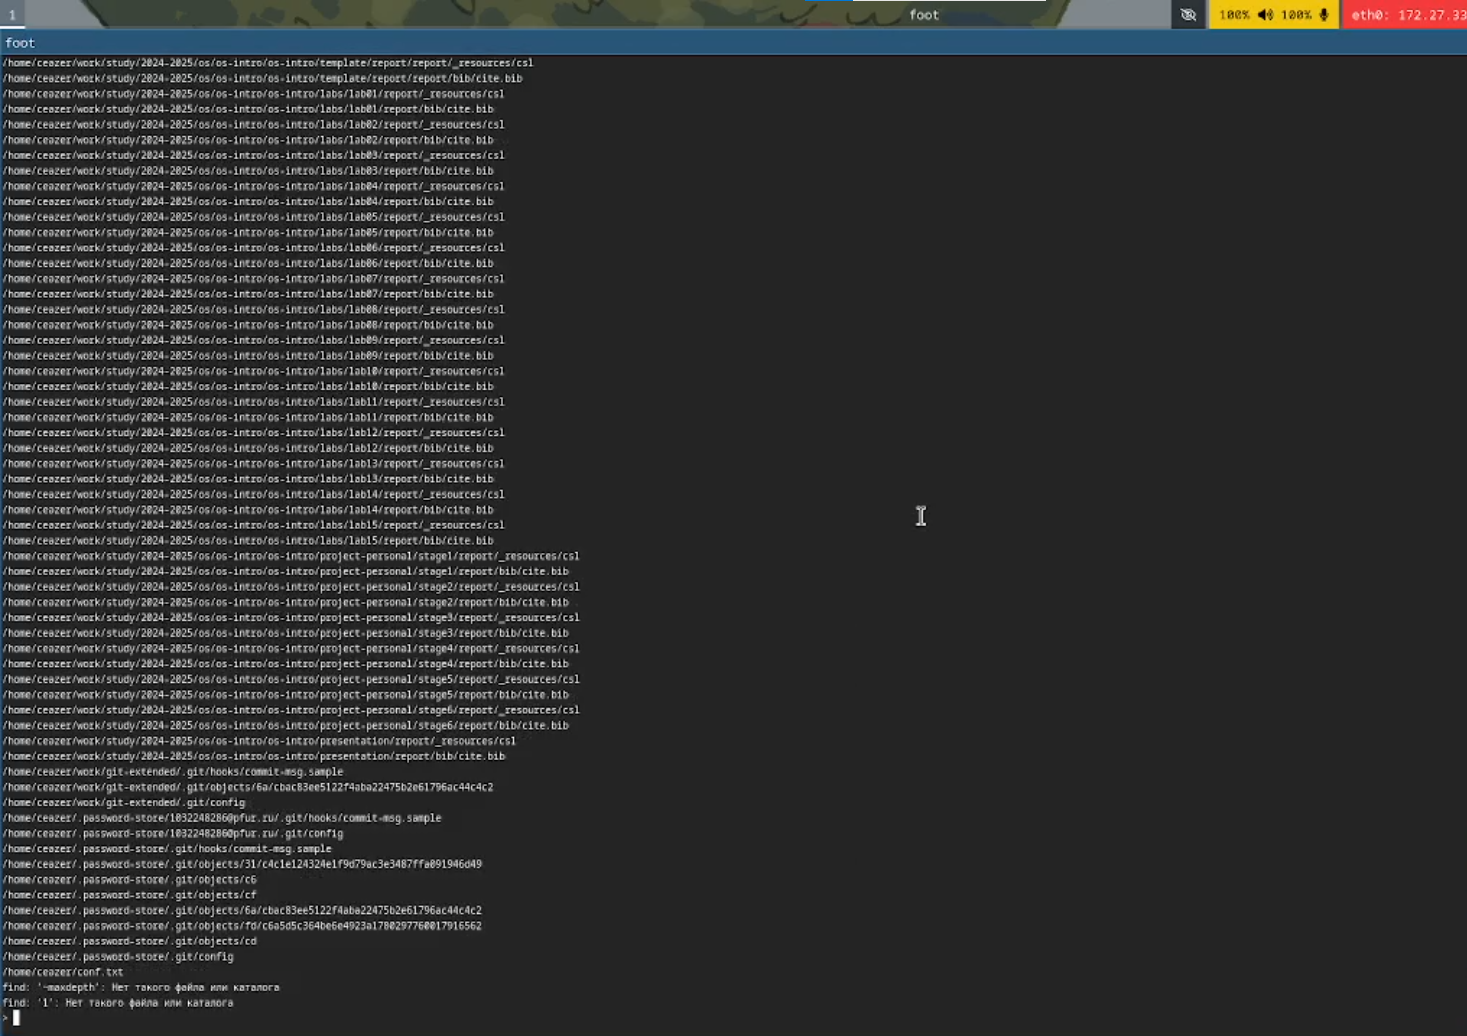
\includegraphics[width=0.8\linewidth,height=\textheight,keepaspectratio]{image/find.png}

}

\caption{Использование команды find}

\end{figure}%
\end{frame}

\begin{frame}{4.3 Работа с текстовым редактором gedit}
\phantomsection\label{ux440ux430ux431ux43eux442ux430-ux441-ux442ux435ux43aux441ux442ux43eux432ux44bux43c-ux440ux435ux434ux430ux43aux442ux43eux440ux43eux43c-gedit}
Создание и редактирование файлов:

\begin{itemize}[<+->]
\tightlist
\item
  Открытие файлов
\item
  Редактирование текста
\item
  Сохранение изменений
\item
  Работа с несколькими файлами
\end{itemize}
\end{frame}

\begin{frame}{4.4 Редактор gedit (скриншот)}
\phantomsection\label{ux440ux435ux434ux430ux43aux442ux43eux440-gedit-ux441ux43aux440ux438ux43dux448ux43eux442}
\begin{figure}[H]

{\centering 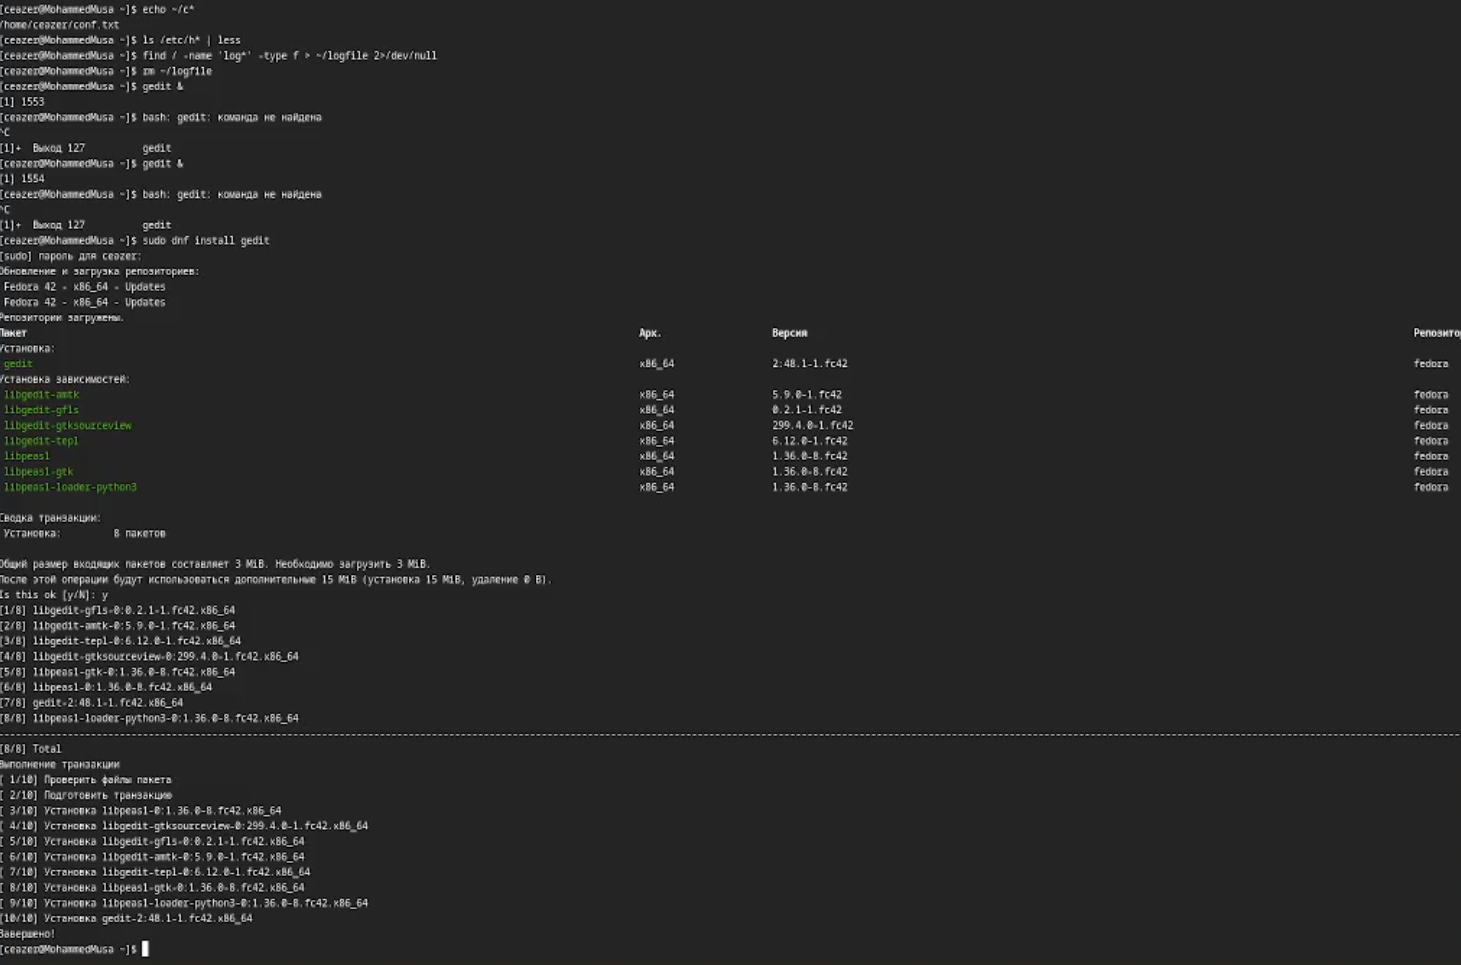
\includegraphics[width=0.8\linewidth,height=\textheight,keepaspectratio]{image/gedit.png}

}

\caption{Работа с редактором gedit}

\end{figure}%
\end{frame}

\begin{frame}{4.5 Управление процессами с kill}
\phantomsection\label{ux443ux43fux440ux430ux432ux43bux435ux43dux438ux435-ux43fux440ux43eux446ux435ux441ux441ux430ux43cux438-ux441-kill}
Завершение процессов:

\begin{itemize}[<+->]
\tightlist
\item
  Просмотр запущенных процессов
\item
  Определение PID процесса
\item
  Отправка сигналов процессам
\item
  Принудительное завершение
\end{itemize}
\end{frame}

\begin{frame}{4.6 Команда kill (скриншот)}
\phantomsection\label{ux43aux43eux43cux430ux43dux434ux430-kill-ux441ux43aux440ux438ux43dux448ux43eux442}
\begin{figure}[H]

{\centering 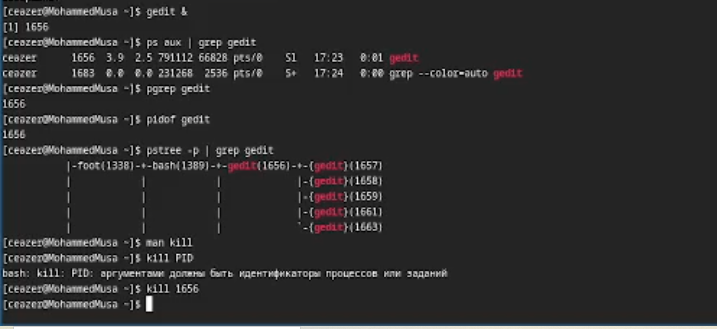
\includegraphics[width=0.8\linewidth,height=\textheight,keepaspectratio]{image/kill.png}

}

\caption{Использование команды kill}

\end{figure}%
\end{frame}

\begin{frame}{4.7 Изучение справочной системы}
\phantomsection\label{ux438ux437ux443ux447ux435ux43dux438ux435-ux441ux43fux440ux430ux432ux43eux447ux43dux43eux439-ux441ux438ux441ux442ux435ux43cux44b}
Работа со справочными страницами:

\begin{itemize}[<+->]
\tightlist
\item
  Просмотр справки по командам
\item
  Навигация по man-страницам
\item
  Поиск информации
\item
  Изучение опций команд
\end{itemize}
\end{frame}

\begin{frame}{4.8 Справочная система (скриншот)}
\phantomsection\label{ux441ux43fux440ux430ux432ux43eux447ux43dux430ux44f-ux441ux438ux441ux442ux435ux43cux430-ux441ux43aux440ux438ux43dux448ux43eux442}
\begin{figure}[H]

{\centering 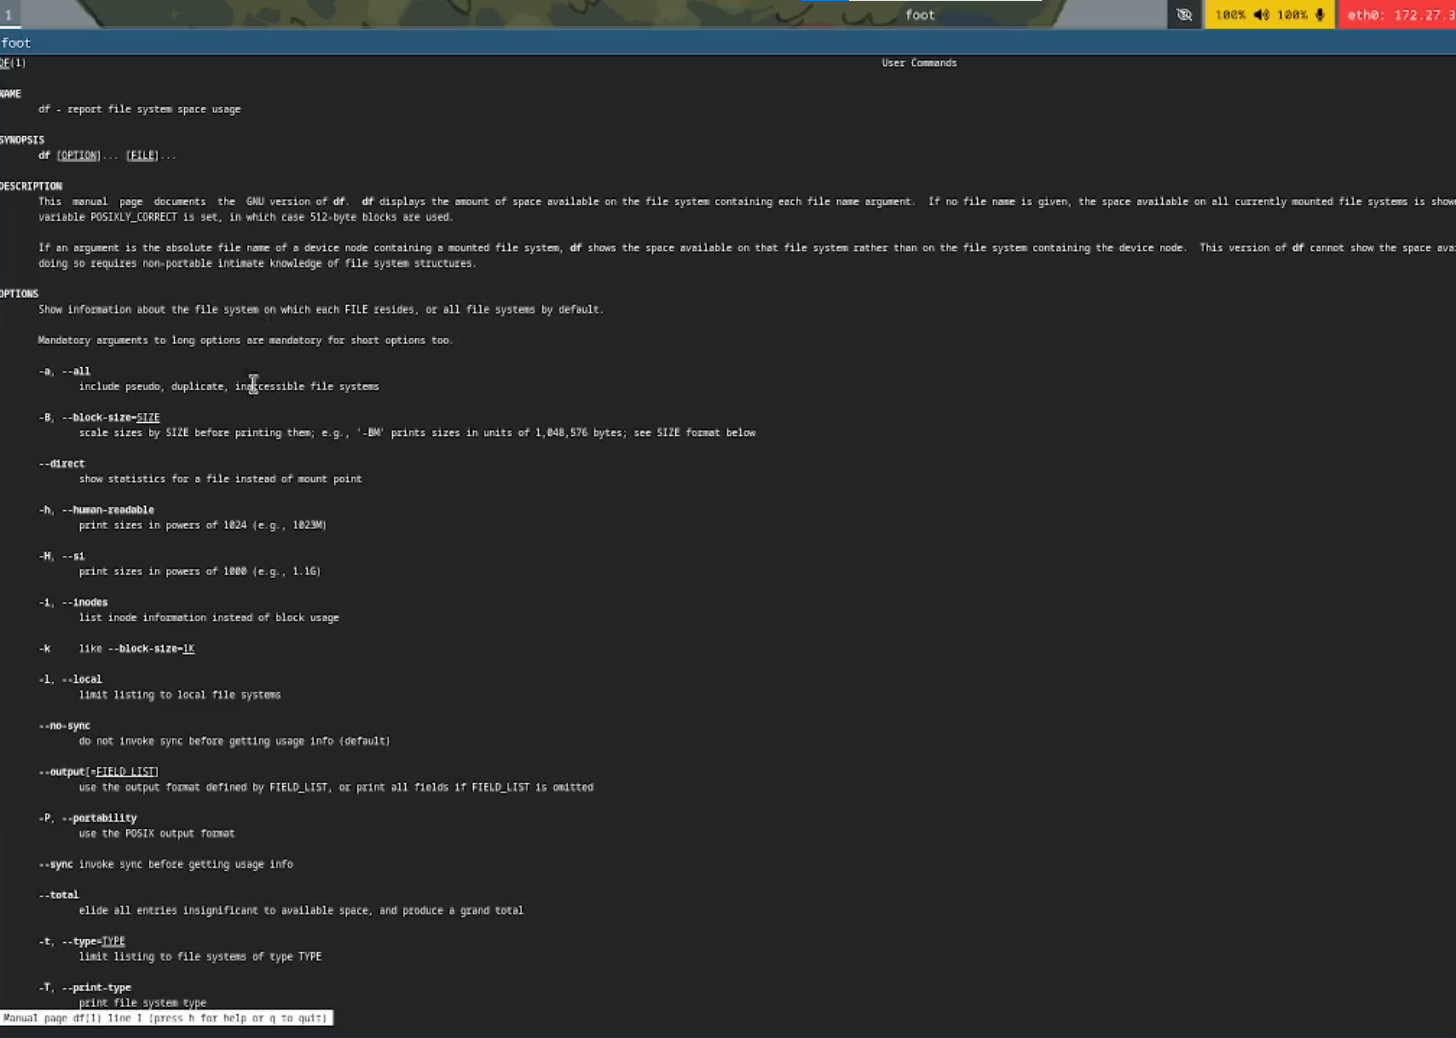
\includegraphics[width=0.8\linewidth,height=\textheight,keepaspectratio]{image/man.png}

}

\caption{Справочная страница команд}

\end{figure}%
\end{frame}

\begin{frame}{4.9 Просмотр дерева процессов}
\phantomsection\label{ux43fux440ux43eux441ux43cux43eux442ux440-ux434ux435ux440ux435ux432ux430-ux43fux440ux43eux446ux435ux441ux441ux43eux432}
Использование pstree:

\begin{itemize}[<+->]
\tightlist
\item
  Отображение иерархии процессов
\item
  Просмотр родительских процессов
\item
  Идентификация дочерних процессов
\item
  Анализ структуры процессов
\end{itemize}
\end{frame}

\begin{frame}{4.10 Дерево процессов (скриншот)}
\phantomsection\label{ux434ux435ux440ux435ux432ux43e-ux43fux440ux43eux446ux435ux441ux441ux43eux432-ux441ux43aux440ux438ux43dux448ux43eux442}
\begin{figure}[H]

{\centering 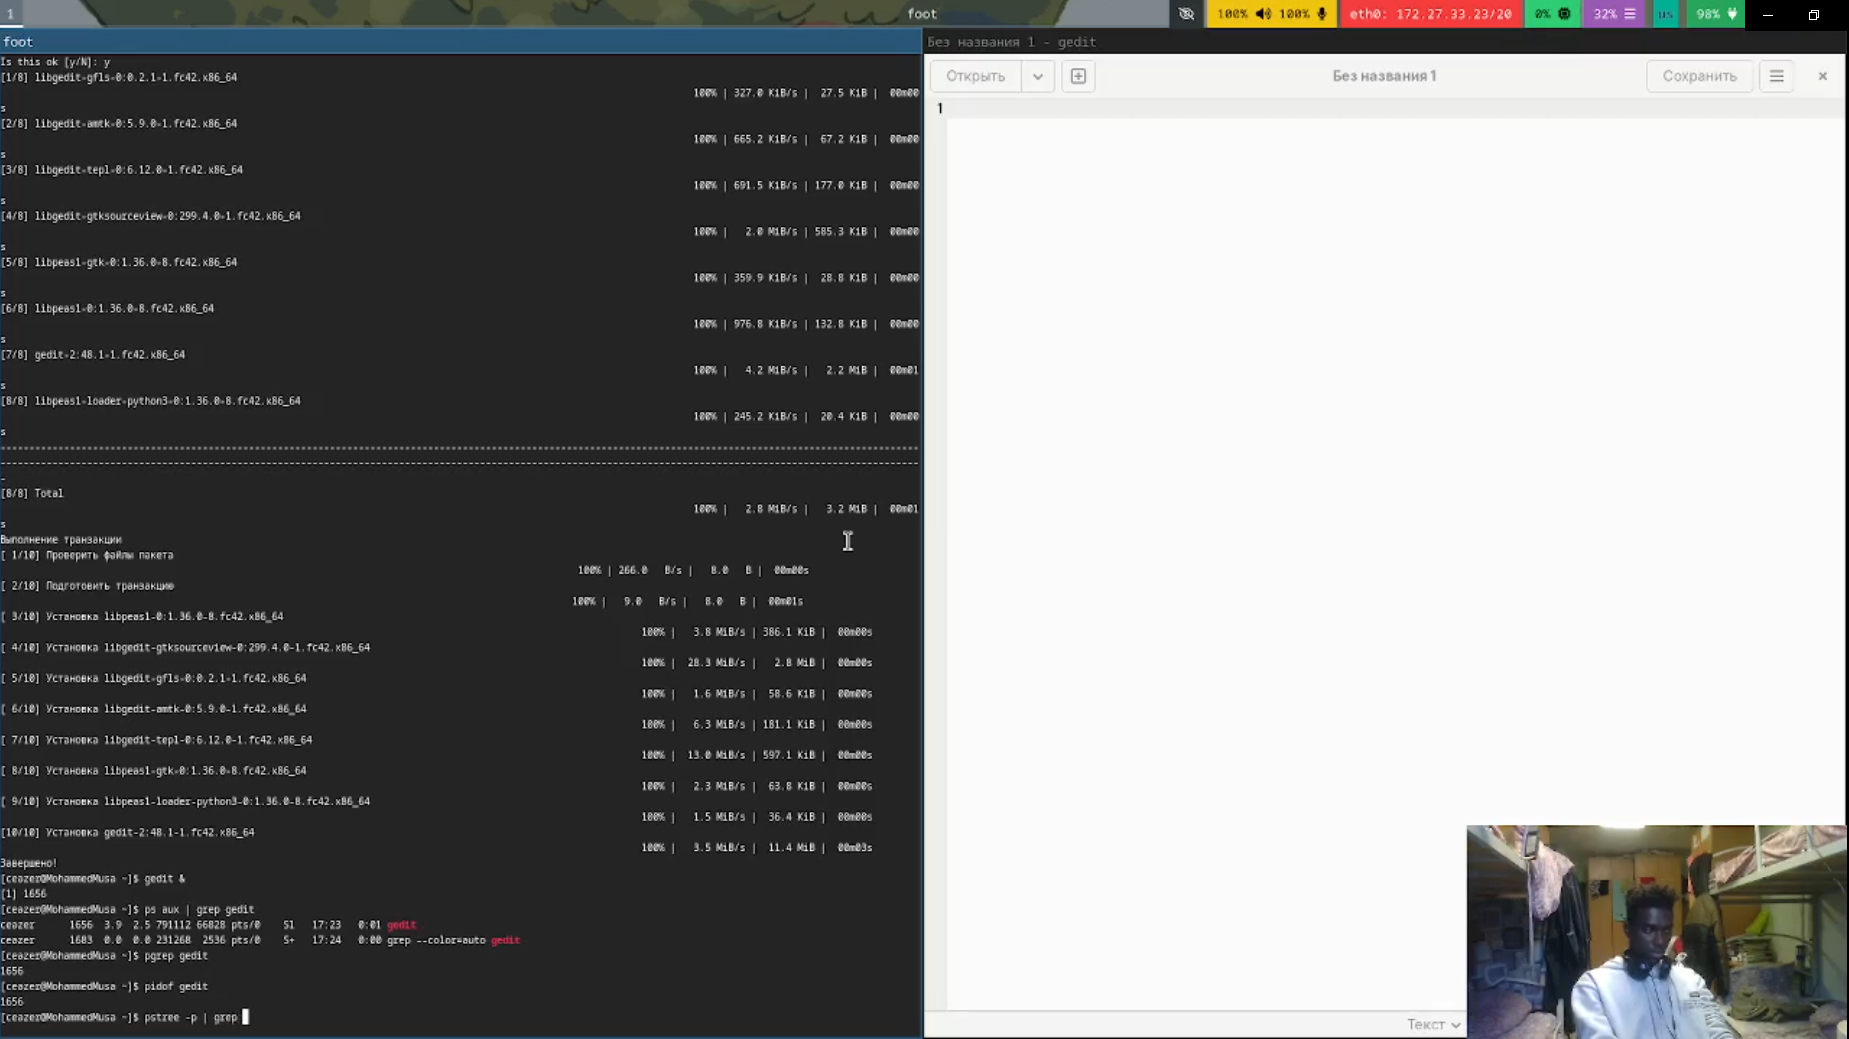
\includegraphics[width=0.8\linewidth,height=\textheight,keepaspectratio]{image/pstree.png}

}

\caption{Дерево процессов}

\end{figure}%
\end{frame}

\begin{frame}{4.11 Результаты выполнения}
\phantomsection\label{ux440ux435ux437ux443ux43bux44cux442ux430ux442ux44b-ux432ux44bux43fux43eux43bux43dux435ux43dux438ux44f}
Финальные результаты работы:

\begin{itemize}[<+->]
\tightlist
\item
  Все команды успешно выполнены
\item
  Процессы управляются корректно
\item
  Файлы найдены и обработаны
\item
  Редактор работает стабильно
\end{itemize}
\end{frame}

\begin{frame}{4.12 Результаты (скриншот)}
\phantomsection\label{ux440ux435ux437ux443ux43bux44cux442ux430ux442ux44b-ux441ux43aux440ux438ux43dux448ux43eux442}
\begin{figure}[H]

{\centering 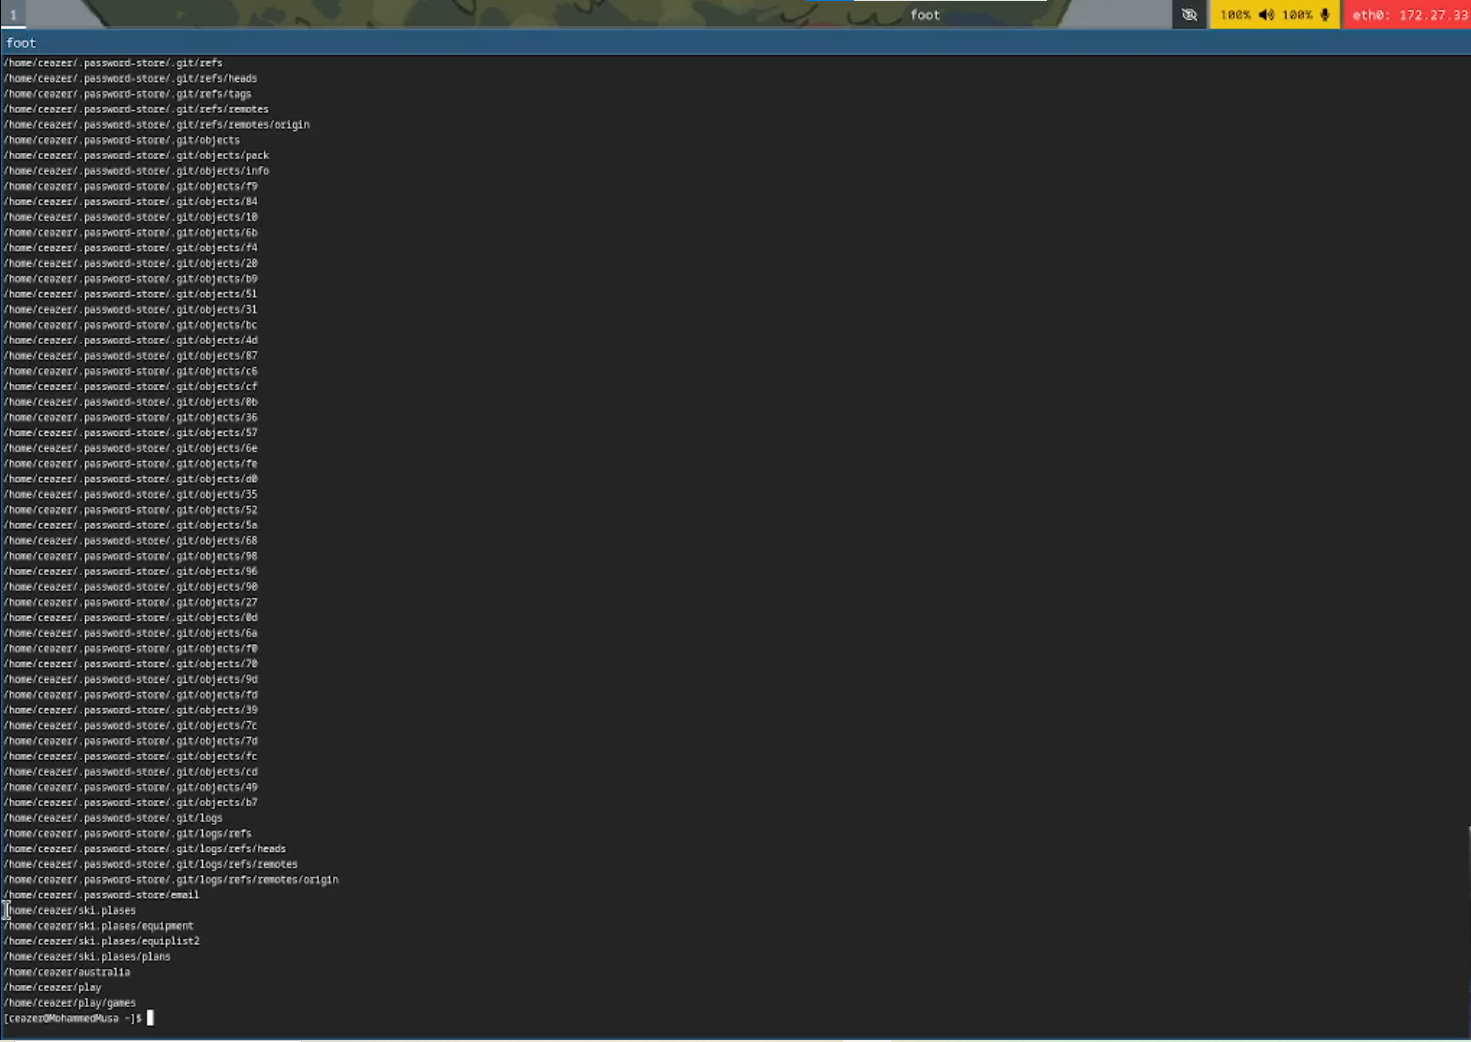
\includegraphics[width=0.8\linewidth,height=\textheight,keepaspectratio]{image/result.png}

}

\caption{Результаты выполнения команд}

\end{figure}%
\end{frame}

\section{5. Результаты}\label{ux440ux435ux437ux443ux43bux44cux442ux430ux442ux44b}

\begin{frame}{5.1 Достигнутые результаты}
\phantomsection\label{ux434ux43eux441ux442ux438ux433ux43dux443ux442ux44bux435-ux440ux435ux437ux443ux43bux44cux442ux430ux442ux44b}
\begin{itemize}[<+->]
\tightlist
\item
  ✅ Освоены команды управления процессами (ps, kill, pstree)
\item
  ✅ Изучено использование текстового редактора gedit
\item
  ✅ Практикован поиск файлов с помощью find
\item
  ✅ Изучена справочная система man
\item
  ✅ Выполнены операции навигации и работы с файлами
\end{itemize}
\end{frame}

\begin{frame}{5.2 Полученные навыки}
\phantomsection\label{ux43fux43eux43bux443ux447ux435ux43dux43dux44bux435-ux43dux430ux432ux44bux43aux438}
\begin{itemize}[<+->]
\tightlist
\item
  Управление процессами в Linux
\item
  Поиск и фильтрация файлов
\item
  Работа с текстовыми редакторами
\item
  Использование справочной системы
\item
  Эффективная работа в командной строке
\end{itemize}
\end{frame}

\section{6. Заключение}\label{ux437ux430ux43aux43bux44eux447ux435ux43dux438ux435}

\begin{frame}{6.1 Выводы}
\phantomsection\label{ux432ux44bux432ux43eux434ux44b}
Освоены важные инструменты Linux:

\begin{itemize}[<+->]
\tightlist
\item
  Процессы --- основа многозадачности в Linux
\item
  Команды ps, kill, pstree --- необходимы для управления системой
\item
  find --- мощный инструмент поиска файлов
\item
  gedit --- удобный редактор для повседневной работы
\item
  man --- незаменимый помощник при изучении команд
\end{itemize}
\end{frame}

\begin{frame}{6.2 Практическое применение}
\phantomsection\label{ux43fux440ux430ux43aux442ux438ux447ux435ux441ux43aux43eux435-ux43fux440ux438ux43cux435ux43dux435ux43dux438ux435}
Изученные инструменты используются для:

\begin{itemize}[<+->]
\tightlist
\item
  Мониторинга и управления системными процессами
\item
  Поиска и организации файлов
\item
  Редактирования конфигурационных файлов
\item
  Диагностики проблем в системе
\item
  Автоматизации задач администрирования
\end{itemize}
\end{frame}




\end{document}
